%\documentclass[12pt, letterpaper, titlepage]{article}
\documentclass[12pt, letterpaper]{article}

\usepackage{amsmath, amsfonts}
\usepackage{booktabs}
\usepackage{amsthm}
\usepackage{graphicx}
\usepackage[margin=1in]{geometry}
\usepackage{hyperref}
\usepackage{cleveref}
\hypersetup{colorlinks = true, linkcolor = blue, citecolor=blue, urlcolor = blue}
\usepackage{natbib}
\usepackage{float}
\usepackage{setspace}
\usepackage{pdfpages}
\usepackage{lineno}
\usepackage{mwe}
\usepackage{comment}
\linenumbers*[1]
% %% patches to make lineno work better with amsmath
\newcommand*\patchAmsMathEnvironmentForLineno[1]{%
 \expandafter\let\csname old#1\expandafter\endcsname\csname #1\endcsname
 \expandafter\let\csname oldend#1\expandafter\endcsname\csname end#1\endcsname
 \renewenvironment{#1}%
 {\linenomath\csname old#1\endcsname}%
 {\csname oldend#1\endcsname\endlinenomath}}%
\newcommand*\patchBothAmsMathEnvironmentsForLineno[1]{%
 \patchAmsMathEnvironmentForLineno{#1}%
 \patchAmsMathEnvironmentForLineno{#1*}}%

\AtBeginDocument{%
 \patchBothAmsMathEnvironmentsForLineno{equation}%
 \patchBothAmsMathEnvironmentsForLineno{align}%
 \patchBothAmsMathEnvironmentsForLineno{flalign}%
 \patchBothAmsMathEnvironmentsForLineno{alignat}%
 \patchBothAmsMathEnvironmentsForLineno{gather}%
 \patchBothAmsMathEnvironmentsForLineno{multline}%
}

% control floats
\renewcommand\floatpagefraction{.9}
\renewcommand\topfraction{.9}
\renewcommand\bottomfraction{.9}
\renewcommand\textfraction{.1}
\setcounter{totalnumber}{50}
\setcounter{topnumber}{50}
\setcounter{bottomnumber}{50}

\newcommand{\jy}[1]{\textcolor{blue}{JY: #1}}
\newcommand{\eds}[1]{\textcolor{red}{EDS: (#1)}}
\newcommand{\of}[1]{\textcolor{violet}{OF: #1}}

% NOTE: To produce blinded version, replace "0" with "1" below.
\newcommand{\blind}{0}

%\title{On Devon Allen's Disqualification at the 2022 World Track and Field 
%Championships} 
%
%\author{Owen Fiore\\
%%   \href{mailto:owen.fiore@uconn.edu}
%% {\nolinkurl{owen.fiore@uconn.edu}}\\
  %Elizabeth D. Schifano\\
  %Jun Yan\\[1ex]
  %Department of Statistics, University of Connecticut\\
%}
%\date{}

\begin{document}
%\maketitle

\if0\blind
{
  \title{\bf On Devon Allen's Disqualification at the 2022 World Track and Field 
Championships}
  \author{Owen Fiore, %\\
%   \href{mailto:owen.fiore@uconn.edu}
% {\nolinkurl{owen.fiore@uconn.edu}}\\
  Elizabeth D. Schifano, %\\
  Jun Yan\\[1ex]
  Department of Statistics, University of Connecticut\\
}
\date{}
  \maketitle
} \fi

\if1\blind
{
  \bigskip
  \bigskip
  \bigskip
  \begin{center}
  {\LARGE\bf On Devon Allen's Disqualification at the 2022 World Track and Field 
Championships}
\end{center}
  \bigskip
} \fi


\doublespace

% Abstract should be under 200 words

\begin{abstract}
Devon Allen was disqualified from the men's 110-meter hurdle final at
the 2022 World Track and Field Championships after recording a
reaction time of 0.099 seconds—just 0.001 seconds faster than the
allowable threshold of 0.1 seconds. This paper explores whether the
reaction times of athletes at the 2022 Championships were unusually
fast compared to other competitions and evaluates the appropriateness
of the 0.1-second disqualification barrier. To investigate these
issues, we employ a rank-sum test for clustered data to compare
athletes' reaction times across multiple competitions, along with a
generalized linear mixed model (GLMM) that accounts for both venue and
heat effects. The results indicate that athletes at the 2022
Championships had significantly faster reaction times on average. This
analysis raises important questions about the validity of the current
reaction time threshold and suggests potential modifications to the
rules that could prevent future disqualifications under similar
circumstances.


\bigskip\noindent{\sc Keywords}:
False Start, GLMM, Hurdle, Reaction Time, Seiko, rank-based test

\end{abstract}

\doublespace


\section{Introduction}
\label{sec:intro}

Devon Allen’s highly anticipated performance at the 2022 World 
Track and Field Championships in Eugene, Oregon, ended in 
controversy when he was disqualified for a reaction time of 
0.099 seconds, just 0.001 seconds below the allowable threshold.
Allen, a University of Oregon alumnus, 
had recently run a time of 12.84 seconds in the 110-meter hurdle 
event, just 0.04 seconds short of the world record. After placing 
third at the U.S. Track and Field Championships, he advanced 
through the preliminary heats and semifinals at the World 
Championships, with reaction times of 0.123 and 0.101 seconds, 
respectively. However, in the final heat, competing in front of his 
home audience, Allen’s reaction time was just 0.001 seconds faster 
than the 0.1-second threshold set by the International Association 
of Athletics Federations (IAAF), resulting in his disqualification, a 
decision that was met with widespread public outcry.


The disqualification of Allen was widely discussed in online 
communities, with some questioning the accuracy of the timing 
equipment. One of the most active platforms was \url{www.LetsRun.com}, 
a website that functions as both a message board and a news outlet. 
The message board, similar to Reddit, is particularly active during 
major running events, including the Olympics and the World Track 
and Field Championships. The news section of the website featured 
articles such as \citet{johnson2022data} and \citet{johnson2022was} 
by Robert Johnson, the site’s founder. Johnson argued that there may 
have been an error with the timing equipment at the 2022 Championships. 
He cited graphs and descriptive statistics, like median reaction 
times, comparing the reaction times at the 2022 Championships to 
those from other competitions, including the U.S. Championships and 
previous World Championships. However, these comparisons lacked formal 
statistical analysis. 


The 0.1-second disqualification threshold in track events has been 
a subject of ongoing debate, with researchers presenting evidence 
both in favor of lowering and raising the
limit. \citet{pain2007sprint} examined
reaction times in nine male athletes and found that the fastest athlete 
had an average reaction time of 0.087 seconds, with a standard deviation 
of 0.004 seconds. Similarly, \citet{komi2009iaaf}, in a study commissioned 
by the IAAF, recommended lowering the disqualification threshold to 0.08 
or 0.085 seconds, arguing that athletes are capable of faster reaction 
times than the current threshold allows. On the other hand, some 
researchers have argued for increasing the threshold.
\citet{brosnan2017effects} suggested raising it to 0.115 seconds based
on data from European and World Championships, while a study of the
2008 Olympics supported the conclusion that athletes cannot reliably
react within 0.1 seconds \citep{lipps2011implications}. Interestingly,
\citet{brosnan2017effects} and \citet{lipps2011implications} relied on
retrospective event data, whereas \citet{pain2007sprint} and
\citet{komi2009iaaf} conducted controlled experiments to assess
reaction time capabilities. The IAAF has not revised the threshold
since its implementation in 1999.


This paper has two primary objectives. First, we investigate whether 
reaction times at the 2022 World Championships were significantly 
different from other competitions, focusing on athletes who competed 
in multiple events. Using a matched-pairs design, we compare reaction 
times across the 2022, 2019, and 2023 World Championships, as well as 
the 2022 national-level competitions. This approach isolates the 
effect of the competition year while controlling for individual 
performance. The clustered nature of the data, with the goal of
assessing differences across events within-athletes, were analyzed
with rank-based comparison approach for clustered data
\citep{datta2005rank}. The second objective is to assess the 
appropriateness of the 0.1-second threshold by modeling reaction 
times from World Championships held from 1999 onward. We use a
generalized gamma distribution with random effects for both venue and
heat in the framework of the generalized additive model for location,
scale, and shape (GAMLSS) \citep{stasinopoulos2024generalized}.
This model estimates the probability of reaction times falling below 
the threshold, helping evaluate the consistency of reaction times and 
whether the current threshold is statistically justified.


The rest of this paper is organized as follows. Section~\ref{sec:Data} 
describes the data collection and datasets used for the two
objectives. Section~\ref{sec:rank} outlines the rank-based comparison
methods for objective~1, rank-based comparison for clustered data with
subunit-level gruping to analyze differences in reaction times
across different competitions. Section~\ref{sec:gamlss} details the
methods for objective~2, the GAMLSS to evaluate the appropriatenes
of the 0.1-second threshold. Section~\ref{sec:Results} presents the
results of both objectives and discusses the implications.
Finally, Section~\ref{sec:concludingremarks} highlights the 
paper’s impact, limitations, and potential for future research.
All data and code for our analysis are provided in the supplementary
materials.



\section{Data}
\label{sec:Data}


This study focuses on reaction times from sprint events where reaction
time plays a critical role. Specifically, we included data from men’s
100-meter dashes and 110-meter hurdles, as well as women’s 100-meter
dashes and 100-meter hurdles. Statistical tests showed no significant
differences in reaction times between these events, supporting their
inclusion in a unified analysis. However, we excluded data from
200-meter dashes and longer events, as their reaction times were found
to be significantly different. This difference is not unexpected, as
reaction time is generally less critical in longer sprint events
compared to shorter distances where explosive starts are paramount.


Two datasets were used to address the study's objectives. To
investigate whether reaction times at the 2022 World Championships
were significantly different from other competitions (Objective 1), we
used data from male athletes in the 110-meter hurdles and 100-meter
dash, and female athletes in the 100-meter hurdles and 100-meter dash,
provided they competed in the 2022 World Championships and at least
one other competition (2022 national championships, 2019 World
Championships, or 2023 World Championships). To assess the
appropriateness of the 0.1-second reaction time threshold (Objective
2), we used reaction times from the 110-meter hurdles and 100-meter
dash across all World Championships held from 1999 to 2023. This
investigation began shortly after the 2022 World Championships, and we
are pleased to include data from 2023, which did not significantly
alter our results \citep{WAData}.


\subsection{Comparison Data with 2022 World Championships}
\label{sec:databeyond}

For assessing the abnormality of the 2022 World Championship, 
the motivation for including data beyond the World Championships arose from 
an exploratory analysis of how United States athletes performed at the 2022 
United States Track and Field Championships, held from June 23--26, 2022, at 
Hayward Field in Eugene, Oregon. Since the same venue hosted the 2022 World 
Championships in August, this provided a unique opportunity to establish a 
baseline for reaction times. 


\subsubsection{2022 National Competitions}
\label{sec:datanational}


\jy{Owen, are there names from 100-m dash?}
To compare reaction times at the 2022 World Championships with those
recorded at national competitions, we constructed a dataset of athletes 
who competed in both settings. Initially, we examined data from four
United States athletes---Trey Cunningham, Daniel Roberts, Grant
Holloway, and Devon Allen---who participated in both the United States 
Track and Field Championships and the World Championships. Each athlete 
recorded faster reaction times in all World Championships races compared 
to their performances at the national-level event. However, this small 
sample size was insufficient for meaningful statistical analysis. To 
expand the dataset, we included reaction times from additional national 
competitions held between May and July 2022 across various countries. 
Compiling this data was challenging, as reaction times were not centrally 
located and often required searching country-specific websites, with many 
results recorded in native languages.


The final dataset consisted of reaction times from athletes who competed 
in both national and international competitions. Reaction times from 
preliminary heats, semifinals, and finals were included to ensure 
sufficient data for analysis. Excluding preliminary heats would have 
significantly reduced the number of athletes and clusters. Each
athlete was considered as a cluster, with observed reaction times
from both the `treatment' group (2022 World Championships) and
the `control' group (national competition) within the cluster. Cluster 
sizes ranged from three to six, with a median size of four. Because gender 
is known to influence reaction times \citep{babicc2009reaction,
  lipps2011implications}, we prepared data for men and women
separately, resulting in 80 reaction times from 17 athletes for each
gender. This setup forms the basis for the rank-based comparison for
clustered data with subunit-level grouping, which accounts for the
within-athlete dependence inherent in this data structure. The top
panel of Figure!~\ref{fig:RankScatterplots} shows the reaction times
of those who competed both at national competitions and the 2022 World
Championships. 


\jy{Could you do a pooled analysis since there is no gender difference
  and event differece in the supplement?}



\begin{figure}[tbp]
  \centering
  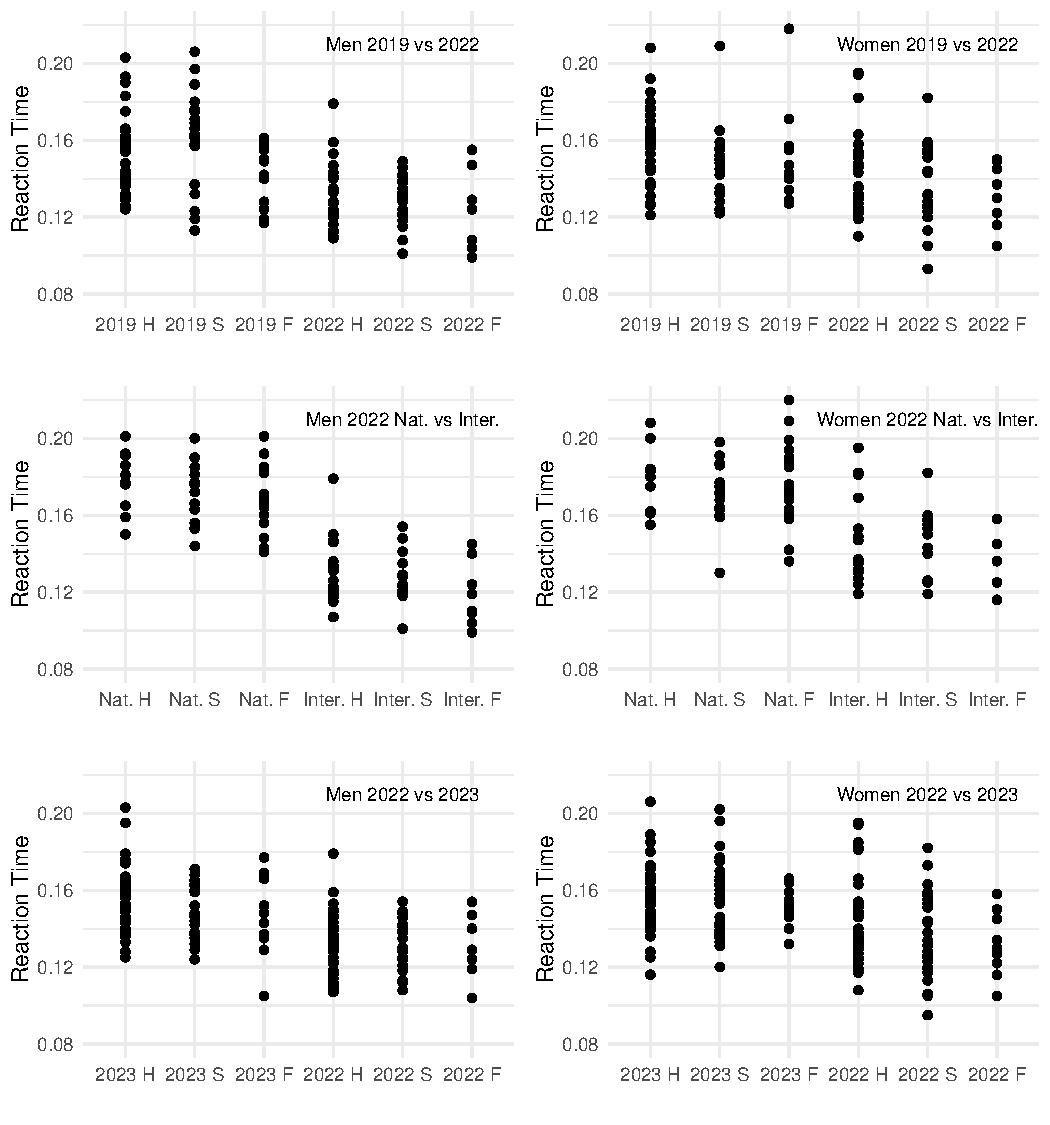
\includegraphics[width=\textwidth]{RankScatterPlots}
  \caption{Reaction times for athletes who competed at the 2022 World Championships
	and at another championship (2022 national, 2019 World, or 2023 World) at which 
	they competed. On the horizontal
  axis below each graph "H", "S", and "F" refer to the heats, semifinals, and 
  finals respectively. Please note that in the last row the 2022 times are to
  the right of the 2023 times.
	\eds{Please check my edited caption; also, I suggest rearranging the rows to 
	use the same ordering as the data was described: put national vs international 
	in first row, 2019 vs 2022 in second row, and 2022 vs 2023 in third row}
	}
  \label{fig:RankScatterplots}
\end{figure}

\subsubsection{2019 and 2023 World Championships}
\label{sec:data2019}

To compare reaction times at the 2022 World Championships with those 
recorded in the 2019 and 2023 World Championships, we prepared datasets 
including reaction times from athletes who competed in the 2022 World 
Championships and at least one of the 2019 or 2023 World Championships. 
Specifically, we identified athletes who participated in both the 2019 
and 2022 World Championships, as well as those who participated in both 
the 2022 and 2023 World Championships. In the 2019-2022 comparison, 
reaction times from 2022 were treated as the `treatment' group, with 
2019 serving as the `control' group. Similarly, in the 2022-2023 
comparison, reaction times from 2022 were treated as the `treatment' 
group, with 2023 serving as the `control' group. This structure allowed 
us to prepare datasets suitable for examining reaction times of athletes 
who competed across multiple World Championships.


Each athlete was treated as a single cluster, containing their reaction 
times from different World Championships. The dataset for the 2019-2022 
comparison contained 134 reaction times from 34 male athletes and 124 
reaction times from 31 female athletes. The dataset for the 2022-2023 
comparison contained 161 reaction times from 45 male athletes and 182 
reaction times from 47 female athletes. While it is theoretically 
possible that athletes improved their reaction times between 2019 and 
2022 or between 2022 and 2023, such improvements are highly unlikely for 
elite sprinters, as they already operate near the limits of human 
performance. Consequently, consistent improvements observed in 2022 
would suggest systematic differences rather than natural variability.


Figure~\ref{fig:RankScatterplots} shows the reaction times of athletes 
who competed in both the 2019 and 2022 World Championships (middle 
panel) and those who competed in both the 2022 and 2023 World 
Championships (lower panel). The athletes included in the 2022 data 
differ between these two comparisons, as the set of athletes who 
competed in both 2019 and 2022 is not the same as the set who competed 
in both 2022 and 2023. To be included, athletes must have competed in 
at least one race at each championship. Notably, Devon Allen recorded 
the fastest reaction times in both the Finals and Semifinals of the 
2022 World Championships, but his disqualification was determined by a 
difference of just 0.002 seconds, with reaction times of 0.101 and 
0.099 seconds, respectively. This highlights the critical role of 
reaction time precision in elite-level competition.

\eds{I also think we need to comment on the men and women's data. But within row
of the figure, don't the distributions appear similar?  If that is so, would a 
reviewer ask why we didn't pool the data for men and women?}
\jy{Let's put the pooled analysis in the supplement.}

\subsection{Data from World Championships 1999--2023}
\label{sec:dataworld}

The data for evaluating the appropriateness of the 0.1-second
threshold was obtained from World Athletics and covers the men's
110-meter hurdles and 100-meter dashes from 1999 to 2023. Due to
possible gender differences \citep{babicc2009reaction,
  lipps2011implications}, data for women's 100-meter hurdles and
100-meter dashes and their analyses were relegated to the
supplementary material. We focus on the reaction times recorded during
semifinal and final heats only, as reaction times from preliminary
heats are often not as fast as those in later heats
\citep[e.g.,][]{collet1999strategic, tonnessen2013reaction,
  brosnan2017effects, zhang2021correlation}. For analysis purposes, we
pooled reaction times from semifinal and final heats to increase sample 
size, which is particularly important for years with limited final heat 
observations. For example, in 2022, only five data points were available 
from the final heat due to two disqualifications and one athlete not 
competing. Unless otherwise noted, this pooled dataset forms the basis 
for our analysis throughout the paper. Additionally, we consider datasets 
that exclude 2022 to assess how our findings might differ when excluding 
this year of interest.


\jy{have the numbers in this paragraph been updated with the
  additional 100-dash data?}
The data is summarized in Figure~\ref{fig:Boxplot}, which presents a
sequence of boxplots of reaction times from 1999 to 2023. It is evident 
that reaction times in 2022 were notably faster, with a median reaction 
time of 0.129 seconds compared to the 0.156 seconds observed in earlier 
studies, such as \citet{brosnan2017effects} for data spanning 1999 to 2014. 
Figure~\ref{fig:Boxplot} also highlights year-to-year variability in 
reaction times, likely influenced by changes in the championship venue 
and environmental conditions such as humidity, precipitation, and 
elevation. Furthermore, advancements in technology and alterations to 
false start rules during the study period may have played a role in these 
variations \citep{willwacher2013novel}.


\begin{figure}[tbp]
  \centering
  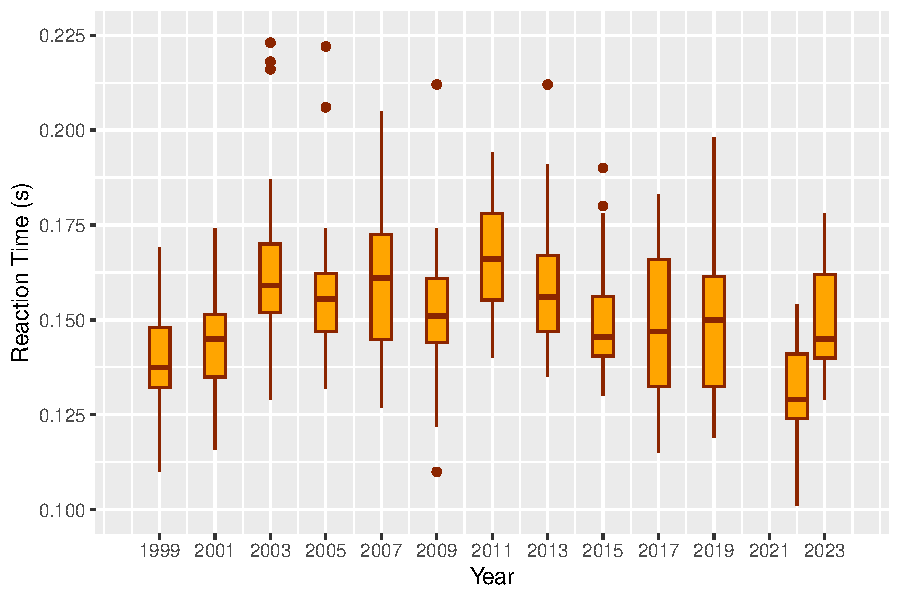
\includegraphics[width=\textwidth]{Boxplot}
  \caption{The reaction times from 1999 to 2023 for the men's 110 meter hurdle
  and 100 meter dash.}
  \label{fig:Boxplot}
\end{figure}


Between 2007 and 2009, World Athletics (formerly the IAAF) allowed one 
false start warning before disqualifying a sprinter \citep{iaaf2009falsestart}. 
This lenient rule led to 18 male and 7 female false starts at both the 2007 
and 2009 World Championships. In 2011, this rule was replaced with the stricter 
policy of automatic disqualification for false starts, aimed at reducing the 
delays caused by repeated warnings. This change reduced men’s false starts 
by two-thirds in 2011, with only six male and four female disqualifications 
\citep{iaaf2009falsestart}. \citet{haugen2013effect} demonstrated that more 
lenient false start rules significantly improved reaction times during the 
1997–2009 period, suggesting that rule changes over the study period may 
have contributed to variations in reaction times across years.


\section{Methods} \label{sec:methods}

The data described in Sections~\ref{sec:databeyond} and~\ref{sec:dataworld} were
analyzed with rank-based methods and a GAMLSS, respectively.


\subsection{Rank-based Comparison}\label{sec:rank}


To test the conjecture that the 2022 World Championships timing device may have 
led to faster recorded reaction times, we compare the reaction times of the same
athletes who have attended both the 2022 World Championships and other 
competitions. 
In this setting, we have clustered data with subunit grouping. In particular,
each athlete is a cluster and the multiple reaction times from the same athlete
can be from either the 2022 World Championships or otherwise.
Let $X_{ij}$ be the $j$th reaction time of athlete~$i$, $i = 1, \ldots, n$,
$j = 1, \ldots, m_i$ where $m_i$ is the number of observations from
athlete~$i$. Let $\delta_{ij}$ be the group indicator of $X_{ij}$; $\delta_{ij}
= 1$ if $X_{ij}$ is in group~1 (2022 World Championships) and $\delta_{ij} = 0$ 
otherwise. Athletes are
assumed to be independent, while subunit observations from the same athlete are
not. The null hypothesis $H_0$ to be tested is that there is no difference
between the two groups; i.e., the distribution of $X_{ij}$ remains the same
regardless of the group indicator $\delta_{ij}$.


\citet{datta2005rank} proposed an extension of the Wilcoxon rank-sum test to
clustered data with subunit-level grouping. The test is designed based on a
within-cluster resampling principle. Consider randomly picking one observation
from each cluster to form a pseudo-sample. Let $X_i^*$ be a random pick from the
$i$th cluster in the pseudo-sample and $\delta_i^*$ its group indicator. The
Wilcoxon rank-sum statistic for the pseudo-sample is
\[
W^* = \frac{1}{n + 1} + \sum_{i=1}^{n} \delta_{i}^{*} R_{i}^{*},
\]
where $R_{i}^{*}$ is the rank of $X_{i}^{*}$ in the pseudo-sample.
The test statistic $S$ is the average of $W^*$ averaged over all possible
pseudo-samples conditioning on the observed data and group indicators.
The mean and variance of $S$ under $H_0$ can be derived so that $S$ can be
standardized to form a $Z$ statistic which follows a standard normal distribution
asymptotically \citep[p.910]{datta2005rank}.


When the sample size is small, the asymptotic normal distribution may
not be reliable, so we also use 1~million random permutations to
simulate the null distribution of the test statistic.
This method is available from the \texttt{clusWilcox.test()} function
with \texttt{method = `ds'} (for \underline{D}atta and \underline{S}atten) and 
\texttt{exact = TRUE} from R package
\texttt{clusrank} \citep{jiang2020wilcoxon}. 


\subsection{GAMLSS}\label{sec:gamlss}

Based on an exploratory analysis, the reaction times are adequately
modeled by a Generalized Gamma (GG) distribution with random effects in
model parameters. The GG distribution has three parameters, denoted by
$\text{GG}(\mu, \sigma, \nu)$ has density function
\begin{equation}
  \label{eq:gg}
f_Y(y \mid \mu, \sigma, \nu) = 
\frac{|\nu| \theta^\theta z^{\theta}}{\Gamma(\theta) y} 
\exp\left(-z \theta\right),
\end{equation}
for $y > 0$, $\mu > 0$, $\sigma > 0$, and $\nu \neq 0$,
where $z = \left(\frac{y}{\mu}\right)^\nu$,
$\theta = 1 / (\sigma^2 \nu^2)$, and
$\Gamma(\cdot)$ denotes the Gamma function.
The GG distribution is highly flexible, encompassing several  
well-known distributions as special cases, such as the
Weibull ($\mu = \nu)$ and  Gamma $(\nu = 1)$ distributions.
Its mean is
\[
  \mu \frac{\Gamma(\theta + 1 / \nu)}
  {\theta^{1 / \nu} \Gamma(\theta)},
\]
provided $\theta > -1 / \nu$. Here,
$\mu$ scales the central tendency, $\sigma$ controls 
dispersion, and $\nu$ determines skewness. This parameterization allows 
the distribution to model asymmetric and heavy-tailed data effectively, making 
it particularly suitable for reaction times.
An implementation of this distribution is available from R package
\texttt{gamlss.dist} \citep{rigby2019distributions}.


Let $Y_{ijk}$ denote the reaction time of observation~$k$ in heat~$j$
of year~$i$. Conditioning on a venue effect $v_i$ for year~$i$ 
and a heat effect $h_{i/j}$ nested within each year~$i$, the
distribution of $Y_{ijk}$ is
$\text{GG}(\mu_{ijk}, \sigma_{ijk}, \nu)$, where
\begin{align}
\log(\mu_{ijk}) &= \beta_0 + v_i , \label{eq:mu}\\
\log(\sigma_{ijk}) &= \gamma_0 + h_{i/j} , \label{eq:sigma}
\end{align}
$v_i$ is normally distributed with mean zero and
variance~$\sigma_v^2$, and $h_{i/j}$ is normally distributed with mean
zero and variance~$\sigma_h^2$.
The two random effects were found useful: one capturing the venue effect, which
is used to contrast years, and the second being the heat effect, where every
race was given a unique identifier with typically five to nine observations
per race. The heat effect is important as it captures the variability in the
amount of time athletes are on the starting blocks before the gun goes off.
This model can be fit with R package \texttt{gamlss}
\citep{stasinopoulos2024generalized}.


Model diagnosis and tail analysis can be done with the fitted GG model
from package \texttt{gamlss}. Normalized quantile residuals, or
z-scores \citep{dunn1996randomized}, of the observations can be
extracted with the \texttt{residuals} method of a \texttt{gamlss}
object. The z-scores can then be checked with a Q-Q plot
\citep{almeida2018ggplot2}. The marginal
distribution of $Y_{ijk}$ is a scale-mixture of GG distributions, which can be
easily simulated from once the parameters are estimated. Many
random numbers generated from the fitted mixture distribution can be used to
approximate the probability of observing a reaction time faster than any given
threshold. We are specifically interested in the probability of a reaction time
being less than 0.1 seconds in order to gauge if that is a reasonable 
disqualification barrier.



\section{Results} \label{sec:Results}

\subsection{Rank-based Comparison} \label{subsec:Results_Rank}

The rank-based methods described in Section~\ref{sec:rank} were used to 
compare reaction times between the 2022 World Championships and other 
competitions in which the same athletes participated. These comparisons 
were conducted separately for men and women, resulting in six total 
comparisons: reaction times from the 2022 national-level championships 
versus the 2022 World Championships for men and women, reaction times 
from the 2019 versus 2022 World Championships for men and women, and 
reaction times from the 2022 versus 2023 World Championships for men and 
women.


\begin{table}
  \centering
  \caption{P-values of comparisons between 
    reaction times from different competitions for the same athletes. 
    2022 Nat. vs Inter. compares reaction times from 2022 national-level 
    championships and the 2022 World Track and Field Championships. 2019 
    vs 2022 compares reaction times from the 2019 and 2022 World Track and 
    Field Championships. 2022 vs 2023 compares reaction times from the 
    2022 and 2023 World Track and Field Championships.}
  \begin{tabular}{c c c c c} 
   \toprule
   Comparison & Permutation & Asymptotic & \# of athletes & \# of observations  \\ 
   \midrule
   2022 Nat. vs Inter. Men & $1.0 \cdot 10^{-6}$ & $ 6.1 \cdot 10^{-5}$ & 17 & 80 \\
   2022 Nat. vs Inter. Women & $1.0 \cdot 10^{-6}$ & $ 1.2 \cdot 10^{-3}$ & 17 & 80 \\[1ex]
   2019 vs 2022 Men & $2.8 \cdot 10^{-5}$ & $1.1 \cdot 10^{-5}$ & 34 & 134 \\
   2019 vs 2022 Female & $ 1.5 \cdot 10^{-3}$ & $6.9 \cdot 10^{-3}$ & 31 & 124 \\[1ex]
   2022 vs 2023 Men & $1.0 \cdot 10^{-6}$ & $1.4 \cdot 10^{-6}$ & 45 & 161 \\
   2022 vs 2023 Female & $1.0 \cdot 10^{-6}$ & $9.4 \cdot 10^{-7}$ & 47 & 182 \\
   \bottomrule
  \end{tabular}
  \label{tab:Clusrankresults}
\end{table}



Table~\ref{tab:Clusrankresults} presents the results from both permutation 
and asymptotic rank-based tests for these six comparisons. The tests reveal 
that the national versus international comparisons yielded the lowest 
p-values, indicating stronger evidence of faster reaction times at the 
2022 World Championships compared to the 2022 national competitions. For 
both men and women, permutation test results were highly significant, 
providing substantial evidence that athletes competing at the 2022 World 
Championships had significantly faster reaction times than they did just 
a few months earlier at national-level events. The comparisons between the 
2019 and 2022 World Championships and between the 2022 and 2023 World 
Championships also produced significant results. Collectively, 
these results suggest that athletes consistently achieved faster reaction 
times at the 2022 World Championships compared to other competitions. This 
finding supports the hypothesis that the 2022 World Championships presented 
conditions conducive to faster reaction times, potentially due to systematic 
or environmental factors.


\subsection{GAMLSS} \label{subsec:Results_GLMM}

\jy{Please add standard errors, which could be from \texttt{summary(gg3b)}}

\jy{Are these numbers correct? I modified with the gg3b in gg.R}

\begin{table}
  \centering
  \caption{Estimated fixed-effect parameters with standard errors in
    parentheses and estimated variance of the random effects from the
    fitted generalized Gamma distribution with venue level random
    effects in $\mu$ and heat level random effects in $\sigma$ in
    Models~\eqref{eq:gg}--\eqref{eq:sigma}.}
  \label{tab:ggfit}
  \begin{tabular}{c c c c c c}
    \toprule
    Data set & $\beta_0$ & $\gamma_0$ & $\nu$ & $\sigma_v$ & $\sigma_h$ \\
    \midrule
    Excluding 2022 & $-$1.910 (0.005)  & $-$2.200 (0.025) & $-$1.177 (0.442) & 0.043 & 0.326 \\
    Including 2022 & $-$1.910 & $-$2.200 & $-$1.178 & 0.058 & 0.320 \\
    \bottomrule
  \end{tabular}
\end{table}


The fitted parameters of the generalized Gamma distribution int he
GAMLSS framework in Equations~\eqref{eq:gg}--\eqref{eq:sigma} are
summarized in Table~\ref{tab:ggfit}. Results obtained from both
excluding and including 2022 data are reported. The fixed-effect
parameters include $\beta_0$, $\gamma_0$, and $\nu$, corresponding to
the intercept of the log-location, log-scale, and shape of the GG
distribution, respectively. Random effects account for variability at
the venue level $\sigma_v$ on the log-scale of the $\mu$ parameter
and at the heat level $\sigma_h$ on the log-scale of the $\sigma$
parameter in the density in Equation~\eqref{eq:gg}. The variance 
of the venue-level random effect is smaller than the heat-level random
effect variance, suggesting that heat-level variability in the scale
parameter is substantial, though on the dispersion parameter. When the
2022 data is included, the fixed-effect estimates remain stable, 
indicating robustness, but the venue-level random-effect variance
increases to 0.0576, reflecting additional variability in the location
parameter, while the heat-level random-effect variance remains stable.
decreases slightly to 0.3198. These results
highlight that reaction times are influenced by both venue and heat-level 
factors, with heat-level variability playing a more prominent role in the scale 
parameter, and that the inclusion of 2022 introduces greater venue-level 
variability, likely due to systematic differences in reaction times that year.


\begin{figure}[tbp]
  \centering
  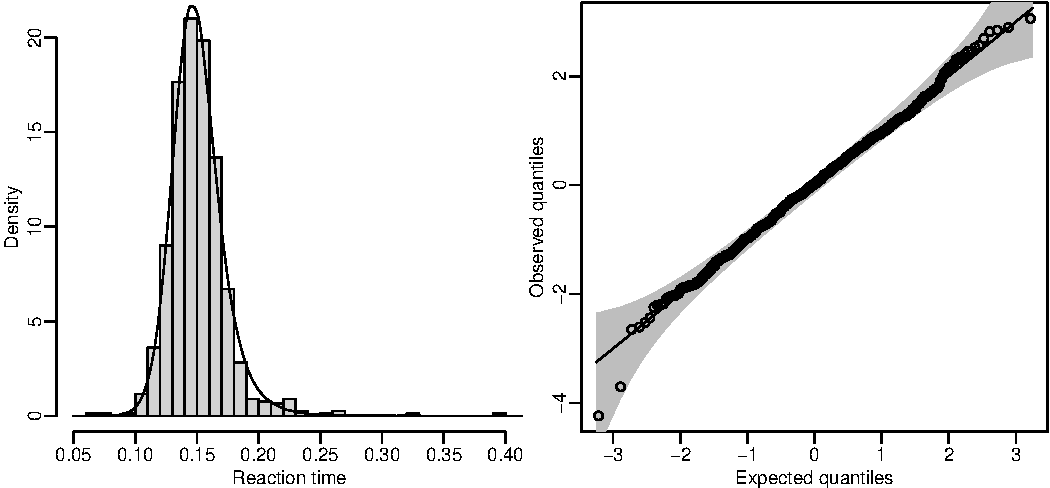
\includegraphics[width=\textwidth]{diagnosis.pdf}
  \caption{Diagnosis of the fitted generalized Gamma distribution with
    random effects in model parameters: kernerl density of 1 million
    observations drawn from the fitted model overlaid with the
    histogram of the observed reaction times (left); Q-Q plot of the
    normal z-score of the quantile residuals from the fitted model.}
  \label{fig:diagnosis}
\end{figure}


Figure~\ref{fig:diagnosis} presents diagnostic checks for the fitted 
generalized Gamma distribution model with random effects. The left 
panel compares the kernel density estimate of one million simulated reaction 
times from the fitted model to the histogram of the observed reaction times. 
The close alignment between the density curve and the histogram suggests that 
the fitted GG model adequately captures the overall distribution of the 
reaction times. The right panel shows a Q-Q plot of the z-scores of the 
quantile residuals from the fitted model. The points lie approximately along 
the 45-degree reference line, indicating that the residuals are consistent 
with the standard normal distribution, supporting the adequacy of the model 
fit. These diagnostics collectively demonstrate that the fitted model provides 
a reasonable representation of the observed reaction time data.


% \begin{figure}[tbp]
%   \centering
%   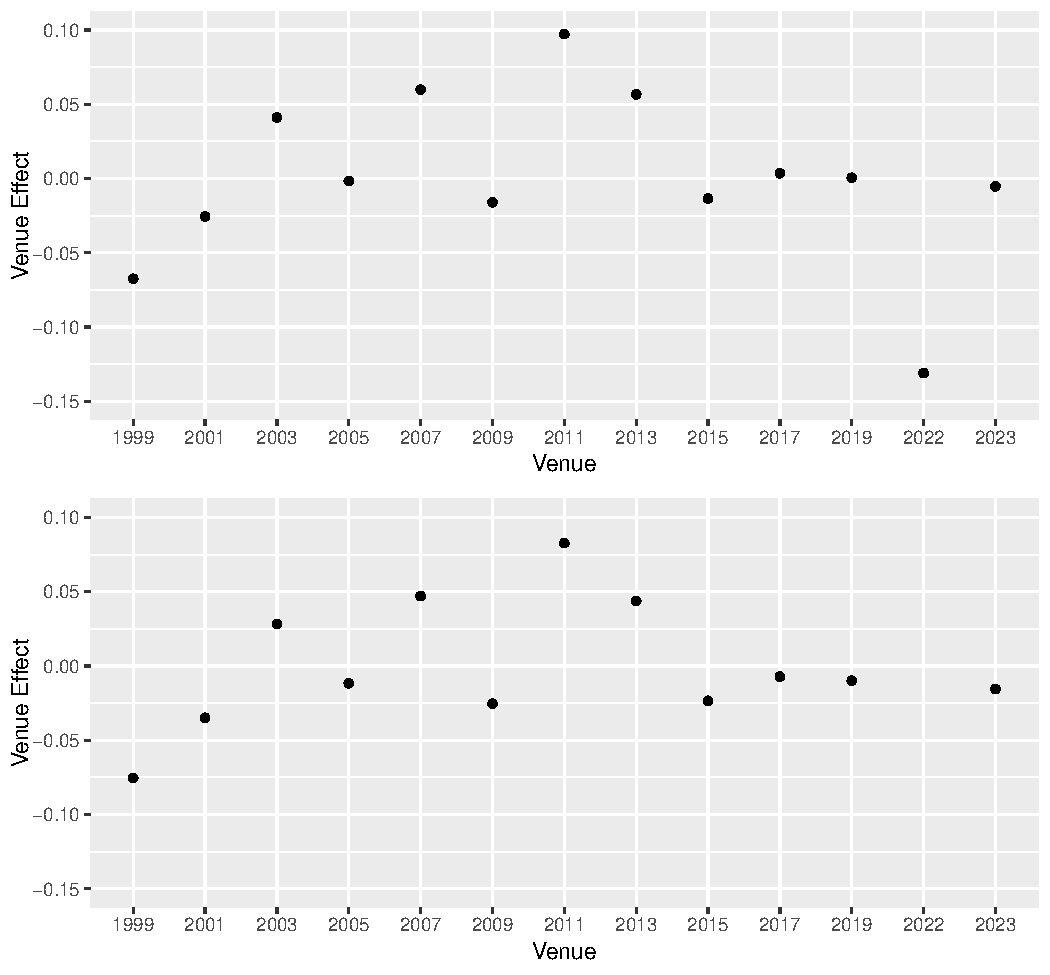
\includegraphics{ComparisonOfVenueEffects}
%   \caption{The venue effects from 1999 to 2023 estimated from the GLMM for the
%     data including 2022 (top) and excluding 2022 (bottom).}
%   \label{fig:VenueEffects}
% \end{figure}

% The uniqueness of 2022 is further demonstrated by Figure~\ref{fig:VenueEffects},
% which shows the values of the venue random effects.  The temporal patterns
% of the two sets of effects look very similar, except that the positive effects
% estimated with 2022 included have higher magnitude than those estimated without
% 2022, which compensates the negative effect of the 2022 with a large magnitude.
% Both plots agree to some extent with the pattern of the boxplots in
% Figure~\ref{fig:Boxplot}. The mismatch is due to the heat effect, since the venue
% effect only captures a smaller part of the variation than the heat effect as
% evident from their standard deviations. It is possible to calculate the extremity
% of the 2022 heat effect as we know that the mean of the heat effects is $0$,
% the standard deviation is $0.42$ as given by Table~\ref{tab:Gamma_parameters},
% and the estimate of the 2022 heat effect is $-0.93$. We find the tail probability
% to be $0.0128$ indicating there is a low chance of observing a venue effect as
% extreme as 2022.


\jy{Could you also test sensitivity for excluding the positive but 
  fault reaction times?}

\begin{table}
  \centering
  \caption{Probabilities of observing reaction times less than threshold 0.08,
  0.09, and 0.10 seconds based on the two effect model.}
  \begin{tabular}{c c c c} 
   \toprule
   Data Set & Threshold 0.08 & Threshold 0.09 & Threshold 0.10  \\ 
   \midrule
   Excluding 2022 & $5.31\cdot10^{-5}$ & $3.53\cdot10^{-4}$ &  $1.94\cdot10^{-3}$  \\ 
   Including 2022 & $6.84\cdot10^{-5}$ & $4.95\cdot10^{-4}$ & $2.76\cdot10^{-3}$ \\
   \bottomrule
  \end{tabular}
  \label{tab:Sim_probability}
\end{table}


The fitted generalized Gamma GAMLSS model with both venue- and heat-level 
random effects provides a framework for assessing how extreme reaction times 
below certain thresholds are. The probability of observing a reaction time 
below a given threshold, assuming no intentional false starts, was approximated 
by generating 10 million realizations from the fitted model. 
Table~\ref{tab:Sim_probability} summarizes the probabilities of observing 
reaction times below 0.08, 0.09, and 0.10 seconds under two scenarios: one 
excluding and the other including data from 2022. Excluding 2022 slightly 
reduces the probability of observing a fast reaction time, but the difference 
is small. For example, the probability of a reaction time below 0.10 seconds 
decreases from $2.76 \cdot 10^{-3}$ (approximately one in 362 starts) to 
$1.94 \cdot 10^{-3}$ (approximately one in 515 starts) when 2022 is excluded. 
Lowering the reaction time threshold from 0.10 to 0.08 seconds drastically 
reduces the likelihood of observing a reaction time below the barrier, with 
the probability dropping from one in every 362 starts (at 0.10 seconds) to one 
in every 14620 starts (at 0.09 seconds) and one in every 146198 starts (at 0.08 
seconds) when 2022 is included. These results highlight the rarity of extremely 
fast reaction times and substantiate the recommendations of \citet{komi2009iaaf} 
to carefully consider the selection of reaction time thresholds.


\begin{table}
  \centering
  \caption{Suggested reaction time barriers based on tail probabilities.}
  \begin{tabular}{c c c} 
   \toprule
   Data Set & Tail probability  $10^{-3}$ & Tail probability $10^{-4}$ \\ 
   \midrule
   Excluding 2022 & $0.096$ & $0.083$ \\ 
   Including 2022 & $0.094$ & $0.082$ \\
   \bottomrule
  \end{tabular}
  \label{tab:Sim_time}
\end{table}

Utilizing the same model, we can determine suitable reaction time barriers 
based on the probability of observing a time below the barrier. As shown in 
Table~\ref{tab:Sim_time}, including the 2022 data suggests a reaction time 
barrier of 0.094 seconds to maintain a 0.1\% chance of observing an 
exceptionally fast reaction time, while a stricter threshold of 0.082 seconds 
is needed to limit this probability to 0.01\%. Excluding the 2022 data results 
in slightly higher thresholds of 0.096 and 0.083 seconds for the respective 
probability levels. These results indicate that while the inclusion of 2022 
data slightly reduces the recommended barrier, the magnitude of the difference 
is relatively small. This approach allows for tailoring reaction time 
thresholds to desired levels of false positive rates, balancing fairness and 
precision in disqualification criteria.


\section{Discussion}\label{sec:concludingremarks}

We set out to answer two questions: were athletes who competed at the 2022 World
Track and Field Championships faster than at other races and is the 0.1 second
reaction time barrier fair.  In regards to the first question, we do believe
that athletes were faster than in comparable meets.  Ideally we would like to
be able to draw data from a central database containing every World Athletics
certified meet which we could use to reference athlete's reaction times.
Unfortunately that is not available at the moment and nearly all of the results
listed on the World Athletics website do not contain reaction times.  The results
of the study could have been stronger if we had been able to look at every race
that athletes like Devon Allen ran in 2022 and analyzed his results at the World
Championship against many other data points.

In addition to the GLMM results results presented above women, the supplementary
file contains results about the women's GLMM results.  We fit a generalized
gamma model to womens 100 meter dash and 100 meter hurdle data from 1999 to 2023
to determine an appropriate reaction time barrier.  We chose to separate these
two studies due to publications suggesting reaction time differences in men and
women.

\of{I think there are some good ideas in these 2 paragraphs but need help
integrating them. Prof Schifano can you help with this?}

The uniformity of the reaction time barrier for both men and women is
perplexing, especially in light of numerous studies that suggest a divergence in
their respective reaction times \citep[e.g.,][]{lipps2011implications,
  babicc2009reaction, panoutsakopoulos2020gender}. These authors posit that
World Athletics may be overlooking inherent gender differences by establishing
an equal reaction time barrier. If gender disparities do exist and 0.1 seconds
is deemed a fair threshold for women, it logically follows that the same cannot
be deemed fair for men, given that the probability of observing sub-0.1-second
reaction times would be inherently higher. \citet{brosnan2017effects} propounds
the adoption of gender-specific reaction time barriers, a stance that appears
logical when considering biological distinctions in reaction times between
genders.


This paper aspires to offer a statistical lens through which to examine Allen's
disqualification at the 2022 World Track and Field Championships, rather than
delivering a conclusive judgment regarding potential equipment malfunction. Our
findings reveal that athletes' reaction times at the event were, in general,
faster than those recorded at other competitions, with
Table~\ref{tab:Clusrankresults} presenting multiple significant p-values that
highlight disparities in average reaction times between the 2022 Championship
and other competitions. Further, our GLMM results indicate that a reaction time
of 0.1-second may not be as exceptional as commonly believed. According to the
probabilities in Table~\ref{tab:Sim_time}, World Athletics might contemplate
adjusting the disqualification barrier to 0.08 seconds, thereby enabling athletes
like Allen to react more swiftly without the apprehension of
disqualification. In summary, while the results designate 2022 as an anomalous
year, Allen's time, despite resulting in disqualification, may not be
categorically extreme.


\section*{Supplementary Material}
The data and R code used for the analysis are available in a compressed file for
ease of reproducibility.

\bibliographystyle{chicago}
\bibliography{citations}


\end{document}
